\documentclass[11pt,a4paper]{article}
\usepackage[utf8]{inputenc}
\usepackage{graphicx}
\usepackage{listings}

%\addtolength{\textheight}{5.5cm}
%\addtolength{\topmargin}{-3.8cm}
\addtolength{\textwidth}{2cm}
\addtolength{\oddsidemargin}{-1cm}

\lstset{language=c++}
\lstset{basicstyle=\footnotesize\ttfamily} %-- => \tiny \scriptsize \footnotesize + \ttfamily \sffamily
\lstset{numbers=left, numberblanklines=true, numberstyle=\scriptsize\ttfamily, stepnumber=1, firstnumber=1, numbersep=7pt, escapeinside={(*}{*)}}
\lstset{breaklines, columns=fullflexible, showspaces=false, showstringspaces=false}
%\lstset{xleftmargin=15pt}
%\lstset{breakindent=0pt, showstringspaces=false, prebreak=|, framexleftmargin=0.4cm}
\lstset{captionpos=b, abovecaptionskip=10pt, belowcaptionskip=10pt, frame=lines, framesep=6pt}

\begin{document}
	
	\title {SpecLib}
	
	\maketitle
	
	\section{specRun function}
	
	This report briefly explains how SpecLib works. The library parallelizes in a speculative fashion loops by chunks. For this purpose, it provides the function
	
	\begin{verbatim}
	specRun(nthreads, begin, end, step, spec_chunk, f, args)
	\end{verbatim}
	
	\noindent which will run a loop from {\tt begin} to {\tt end} with step {\tt step} whose body is given by the function {\tt f} using {\tt nthreads} threads. The first argument of function {\tt f} must be the index of the loop, while the remaining argument must be C++ references to the data on which the execution is speculative, that is, the data that can be modified by the loop body in ways that make the computation not safe to be executed in parallel and which can thus make the speculation fail. The variables on which the execution is speculative are provided to {\tt specRun} as the arguments {\tt args} after function {\tt f}. They must be provided in the same order that function {\tt f} expects them.
	
	The function splits the loop in chunks of {\tt spec\_chunk} consecutive iterations, and for each one, it executes three kinds of tasks:
	\begin{description}
		\item[a sequential task] that runs in a single thread in sequence all the iterations of the chunk.
		\item[a parallel task] that evenly divides the iterations of the chunk on the threads available, giving place to subchunks that are executed in parallel, one per thread.
		\item[a validation task] that is run when the two previous have finished, which compares the value of the speculative data of the sequential and the parallel task in order to determine whether the speculation was successful.
	\end{description}
	
	Since the parallel version of a chunk usually finishes before the sequential one, as soon as the parallel version finishes, it triggers the execution of the next chunk, also using the three tasks described. Notice that when {\tt specRun} runs the first chunk of the loop, its results are necessarily correct, as they correspond to a sequential execution on the original valid data of the application. Nevertheless, in the case of a subsequent loop chunk both the sequential and the parallel tasks are speculative, as they operate on data computed by the parallel version, which can be thus valid or not, the outcome being unknown until the validation task is run. For this reason, when a validation is unsuccessful, {\tt specRun} has to terminate and disregard the results of all the tasks associated to later chunks, and restart the execution of the loop from the last valid chunk computed.
	
	Figure~\ref{fig:spec_execution} illustrates the operation of the library with a loop with four chunks in an execution using four threads. Each row in the figure represents the tasks executed by a different thread. The task Sc$n$ executes in a single thread the chunk $n$, while the tasks Pc$n$ represent the parallel execution on that chunk on the threads available when the parallel execution begins. For this reason, while the first chunk can use three threads for the parallel execution, the other one being busy with Sc1, the parallel execution of the second chunk can only exploit two threads, as another one must be devoted to executing Sc2. The small V$n$ tasks perform the validation that compares the results of Sc$n$ and Pc$n$. In the figure we assume that while V1 was successful, this was not case for V2. Since this implies that the correct values computed by Sc2 were different from the speculative ones computed by Pc2, and Sc3 started from these latter speculative values, {\tt specRun} must terminate the Sc3 that was being executed and restart it with the valid values computed by Sc2. Notice also that when Pc2 finished there were only two threads available, and in that situation it was impossible to run a parallel version of the chunk number 3, as after launching Sc3 there was only one thread left. As shown in the figure, in these situations the library only runs the sequential task. We can see however that after V3 terminated the Sc3 in curse, four threads were available again. Therefore {\tt specRun} could devote one of them to the restarted Sc3 and the other three ones to Pc3. All the remaining validations are assumed to be successful in the figure.
	
	\begin{figure}[t]
		\begin{center}
			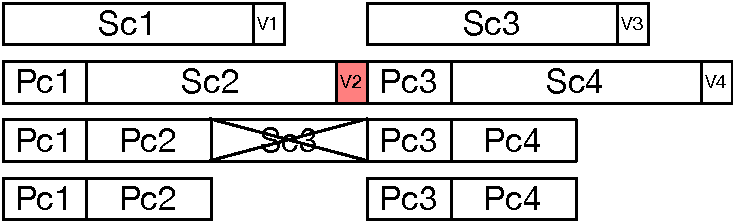
\includegraphics[width=0.75\textwidth]{SpecLib.pdf}
			\caption{Example of parallel execution of 4~chunks on 4~threads using SpecLib}\label{fig:spec_execution}
		\end{center}
	\end{figure}
	
	The programming overhead of {\tt specRun} is very small. For example, the speculative parallelization of a simple loop to compute the maximum value in a vector, which can be performed sequentially as
	
	\begin{verbatim}
	for (int i = 0; i < N; i++) {
	if (Vals[i] > max) {
	max = Vals[i];
	}
	}
	\end{verbatim}
	
	\noindent can be expressed, using {\tt t} threads and chunks of {\tt c} iterations as
	
	\begin{verbatim}
	specRun(t, 0, N, 1, c, [&](int i, int& r) {
	if (Vals[i] > r) {
	r = Vals[i];
	}
	}, max);
	\end{verbatim}
	
	While as we have seen, the function proposed as argument for {\tt specRun} only executes a single iteration of the loop, it is also possible to use a function that rans at once a block of iterations. In this case, before the speculative arguments, the function should receive, in this order,
	\begin{enumerate}
		\item a {\tt const SpecLib::CommonSpecInfo\_t\&} object that can be used to detect whether the chunk execution is cancelled by invoking its method {\tt cancelled()}. This can be useful to exit the chunk execution as soon as possible in case on cancellation.
		\item the beginning of the chunk
		\item the end of the chunk
		\item the step of the loop
	\end{enumerate}
	The following code exemplifies the speculative parallelization of the same loop using this second kind of function:
	
	\begin{verbatim}
	specRun(t, 0, N, 1, c, [&](const SpecLib::CommonSpecInfo_t& cs, 
	int begin, int end, int step, int& result) {
	for (int i = begin; (i < end) && !cs.cancelled(); i+=step) {
	if (Vals[i] > r) {
	r = Vals[i];
	}
	}
	}, max);
	\end{verbatim}
	
	The data on which the speculation is performed can be any object that provides deep copies, assignments and the comparison operator {\tt !=}. 
	
	
	\section{SpecConsecVector class}\label{sec:SpecConsecVector}
	
	A potential performance problem for large objects such as arrays is that even if the iterations performed speculatively in each chunk only modify a portion of their content, {\tt specRun} does not know this and it has thus to copy and verify the whole object. As an added optimization, SpecLib provides a class template {\tt SpecConsecVector<T>} that allows to avoid this performance problem for the common situation that iteration $i$ of the loop only modifies element $i$ of a vector of elements of type {\tt T}. This kind of object can be built from pointers and standard array representations of C++ such as {\tt std::vector} or {\tt std::array}, and the only thing the user needs to do is to use it as argument and associated formal parameter for the speculative function {\tt f} provided to {\tt specRun}.
	
	In order to illustrate this optimization, let us assume we want to compute the maximum element in a vector {\tt Vals} and also store in each element $i$ of an output vector {\tt result} the maximum value found up to that point $i$ in {\tt Vals}. We can express this sequentially as
	
	\begin{verbatim}
	for (int i = 0; i < N; i++) {
	if (Vals[i] > max) {
	max = Vals[i];
	}
	result[i] = max;
	}
	\end{verbatim}
	
	The optimized speculative version using {\tt t} threads and chunks of {\tt c} iterations, expressed with SpecLib would be
	
	\begin{verbatim}
	specRun(t, 0, N, 1, c, [&](int i, int& r, SpecConsecVector<int>& rv) {
	if (Vals[i] > r) {
	r = Vals[i];
	}
	rv[i] = r;
	}, max, SpecConsecVector<int>(result));
	\end{verbatim}
	
	
	\section{SpecVector class}
	
	Unfortunately, in many codes modifications on arrays happen with patterns that cannot be easily described, for example because they use indirections or complex indexing functions. For this case the library provides a data type {\tt SpecVector<T, I>} that has the same purpose as {\tt SpecConsecVector}, but which supports total flexibility in the indexing of the array it represents. This is achieved though at the cost of much higher storage and management overheads. In this class {\tt T} represents the type of the elements stored in the array, while {\tt I} is the type of the indexes used to access the array. Specifying {\tt I} is optional, the default being {\tt std::size\_t}. 
	
	The constructor of an {\tt SpecVector} admits three arguments:
	\begin{enumerate}
		\item compulsory: pointer to the array. As in the case of the {\tt SpecConsecVector}, it can be either a raw pointer, a {\tt std::vector} or a {\tt atd::array}.
		\item compulsory: upper bound of the number of different elements of the array that can be modified/written during the execution of a single speculative chunk of iterations. Even if we are sure about the exact value of this number of elements, we should provide a number slightly larger for this argument ir order to make sure that the execution is successful. If the number provided is exceeded during the execution of some chunk of iterations, the library will break throwing an exception. 
		\item optional: ratio between (a) the size for the storage of the array elements modified during the execution of a chunk specified as second argument and (b) the size of the internal hash table used to locate the elements in that storage. If it is not specified, it defaults to 1. Larger ratios lead to proportionally smaller hash tables and more expensive search processes, as there will be on average proportionally more elements mapped to the same hash table entry.
	\end{enumerate}
	
	Let us consider again the code that was used in Section~\ref{sec:SpecConsecVector} to illustrate the use of the {\tt SpecConsecVector}:
	\begin{verbatim}
	for (int i = 0; i < N; i++) {
	if (Vals[i] > max) {
	max = Vals[i];
	}
	result[i] = max;
	}
	\end{verbatim}
	
	In this code it is clear that each iteration writes to a single element of the array {\tt result}. As a result we know that in a chunk of {\tt c} iterations, at most {\tt c} different elements of {\tt result} will be modified. Let us imagine that we are not able to realize that a {\tt SpecConsecVector} can be used to perform the speculative parallelization of this loop and we have to rely instead on the generic {\tt SpecVector}. In this case, we could speculatively parallelize the execution of the loop using {\tt t} threads and chunks of {\tt c} iterations as
	
	\begin{verbatim}
	specRun(t, 0, N, 1, c, [&](int i, int& r, SpecVector<int>& rv) {
	if (Vals[i] > r) {
	r = Vals[i];
	}
	rv[i] = r;
	}, max, SpecVector<int>(result, c + c/20 + 2));
	\end{verbatim}
	
	Let us notice how in the constructor of the {\tt SpecVector} we have not provided the exact number {\tt c} of elements written in a chunk of {\tt c} iterations, but a slightly larger value, as advised in the description of the constructor.
	
	It is very important to realize that {\tt SpecVector} will count as potentially modified any element accessed through a non-{\tt cost} reference or pointer to the object; even if that element is never modified. This means that if the following function is used as argument to {\tt specRun} to represent the code to execute for one iteration of a loop:
	
	\begin{verbatim}
	void f(int i, SpecVector<double>& v, int& max) {
	if(v[i] > max) {
	const double tmp = max;
	max = v[i];
	v[i] = tmp;
	}
	}
	\end{verbatim}
	
	\noindent the library will count one element written in {\tt v} in every iteration of the loop, even if this only happens when {\tt v[i] > max}. This can be avoided by making non-modifying accesses through a {\tt const} reference to the object: 
	
	\begin{verbatim}
	void f(int i, SpecVector<double>& v, int& max) {
	if(const_cast<const SpecVector<double>&>(v)[i] > max) {
	const double tmp = max;
	max = v[i];
	v[i] = tmp;
	}
	}
	\end{verbatim}
	
	In fact, since accesses to the object are very expensive, we should try to minimize them, for example by rewriting the function in this way:
	
	\begin{verbatim}
	void f(int i, SpecVector<double>& v, int& max) {
	const double val = const_cast<const SpecVector<double>&>(v)[i]; 
	if(val > max) {
	const double tmp = max;
	max = val;
	v[i] = tmp;
	}
	}
	\end{verbatim}
	
	Just as the previous one, this implementation counts as written the minimum posible number of written elements; but it makes fewer accesses to the object. Still, it has the drawback that it requires two accesses to the vector in the iterations where it is updated. For this reason, even if it requires counting one element of the array as written in every iteration, the following implementation, which always makes a single access per iteration, might provide better performance in situations in which the code often updates the array:
	
	\begin{verbatim}
	void f(int i, SpecVector<double>& v, int& max) {
	double& val = v[i];
	if(val > max) {
	const double tmp = max;
	max = val;
	val = tmp;
	}
	}
	\end{verbatim}
	
\end{document}

